In order to create a representative sample of the workload, we need to identify patterns in the query log. The task of identifying patterns directly from the log is difficult. A naive approach would be to consider individual queries as atomic components of the query logs and cluster them by directly extracting features. The most important difference between a smartphone database workload and that in database servers are the users' bursts of activity. Most benchmarks like the TPC-C focus on emulating homogenous query workloads of an OLTP system. Their goal is to analyse throughput fpr these homogenous workloads. But it is not correct to truly emulate smartphone query workloads without emulating the inermittent bursts of query activity. These bursts can only be detected by looking at the chronological attributes like query timestamp and query interarrival time. This approach does not consider the chronological ordering of the queries. Hence, This naive clustering is not meaningful. Another level of abstraction is needed to extract meaningful patterns from the query log.

\begin{figure*}[h!]
    \centering
    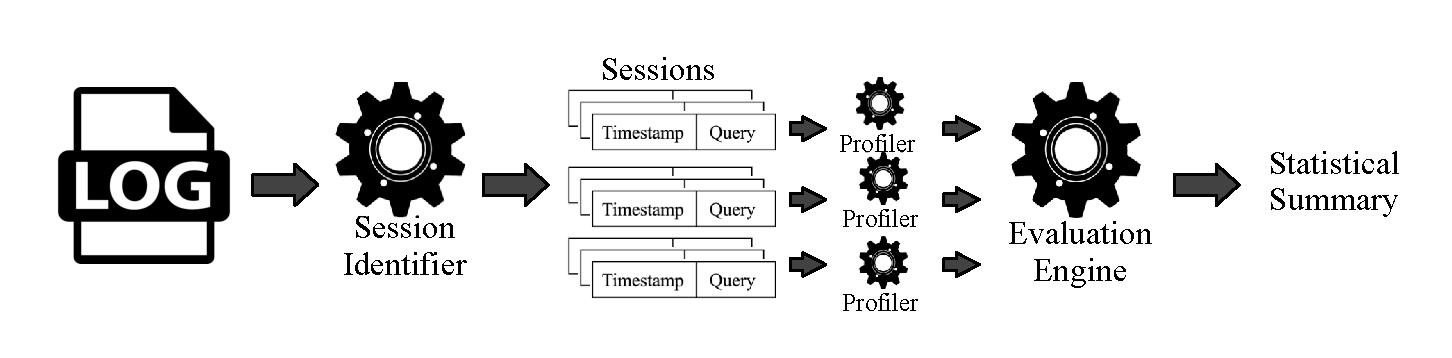
\includegraphics[width=\textwidth]{graphics/approach}
    \caption{Abstract views of inputs and outputs of both approaches}
    \label{fig:approaches}
\end{figure*}

We introduce the concept of sessions to solve this problem. A user would interact with their smartphone multiple times a day for small intervals of time. These bursts of intermittent activity are captured in database user sessions. These form the atomic units of the query log which can be used for detecting patterns. 

A logical task, called an \emph{activity}, performed by a user on a smartphone, such as checking for new email, might produce multiple queries to the database. Since smartphone applications keep switching between foreground and background, these queries could be arbitrarily spaced out in time. Hence, one database user session might contain one or more logical user tasks. A logical user task might be spread across multiple database user sessions. These sessions are useful in capture subset of logical tasks which are repetitive. Since there is no discrete indicator of the start and end of a database user session in smartphones, we use a heuristic to help define one. If queries in a log are apart in time beyond a threshold, we consider them to be a part of different sessions.

After partitioning the query log into \emph{sessions}, we create a statistical summary of \emph{similar} activities by providing frequencies of each pattern detected. This could be done in two ways: (1) Supervised approach, and (2) Unsupervised approach.

\subsection{Supervised Approach}
\label{sec:supervised}
We present the supervised approach as a method that requires human intervention, and extensive effort since it requires the activity data to be collected and labeled.

In this approach, we define a set of atomic activities that are possible to be performed on a mobile app, and look for them every time a user uses the phone. The frequency of the activities that appear together or individually in these \emph{sessions} provide an outlook of how a user utilizes an application. The process is illustrated in Figure~\ref{fig:approaches}.

\todo{Go on. Describe the figure.}

\begin{figure}[h!]
    \centering
    \includegraphics[width=0.45\textwidth]{graphics/supervised}
    \caption{Analysis box of the supervised approach}
    \label{fig:supervised}
\end{figure}


\subsection{Unsupervised Approach}
\label{sec:unsupervised}

Our main contribution in this paper is the unsupervised approach, which eliminates the human intervention and effort required. The criteria for this approach to be successful is to be able to have comparable performance with the supervised approach.

With this approach, we take the workload as the only input, and look for the behavior of the user when they take the phone in their hands every time on a typical day. The frequency of certain types of queries that appear together or individually in a user session provides a summary of the expected user activity.  This process is illustrated in Figure~\ref{fig:approaches}.

\todo{Go on. Describe the figure.}


Both the supervised and unsupervised approaches described in the previous section has three blackboxes: (1) Session identifier, (2) Profiler, and (3) Analyzer. In this section, we describe the methods that we applied to implement these black boxes.






%% I COMMENTED OUT THE REST OF THE SECTION. WE WILL INTRODUCE CLUSTERING LATER - GOKHAN %%

%Even though we have now obtained an atomic unit of a query log for the purpose of detecting patterns, the problem of poor clustering owing to directly extracting features still remains to be addressed. We introduce another level of abstraction to segregate queries based on their interest over database attributes. This is determined by similarity in their semantic structure. Since most of the queries issued to a smartphone database are made through ORMs, they contain ingerent structure. Each query can belong to one of many query clusters. This makes the detection of patterns easier.  

%To summarize, we perform a two step preprocessing : Clustering and Session Identification. Our system operates in three stages: (1)~A \textbf{clustering} phase where the queries in the log are segregated by similarity in their semantic structure, (2)~A \textbf{session identification} phase where the query logs are partitioned based on the timing of queries to identify the length and coverage of individual user sessions, and (3)~A \textbf{session parameter detection} phase where the partitioned sessions are inspected in order to establish associations of what kinds of activities are performed together in a typical session, as well as detection of unusual activities. These stages are illustrated in Figure~\ref{fig:abstractview}. 

%\begin{figure}[h!]
%    \centering
%    \includegraphics[width=0.5\textwidth]{graphics/systemoutline}
%    \caption{Abstract view of inputs and outputs. (a) Clustering (b) Session Identification}
%    \label{fig:abstractview}
%\end{figure}


%\subsection{Clustering phase}

%The query workload created by an Android application consists of queries generated by user activity. Most of the applications support several functionalities, and these functionalities generate queries with conditions based on the user needs.

%In this phase, we aim to distinguish these functionalities based on the variety of structural differences in queries. We observe and process every SQL query issued to the mobile DBMS. We extract the relevant features of the query considering what kind of attributes the query is accessing with that particular query. Our work follows the basic SQL query feature extraction principles of Makiyama \textit{et al.}~\cite{makiyama2015text}. Using these query features, we construct a feature vector for each query to cluster similar queries together. We use hierarchical clustering since there is not a specific number of clusters we need. This step provides us with the information required to see frequency of different kinds of queries a user issues.

%\subsection{Session identification phase}
%The usage pattern of databases in smartphones differs significantly from the continuous patterns experienced in database servers~\cite{kennedy2015pocket} or more traditional computing devices like PCs.  

%Typically, an end user would use their smartphones multiple times a day for small intervals of time. This pattern of intermittent bursts of activity motivates a new way of looking at these usage patterns. Identification of patterns would require breaking down the workload into logical units which can be compared for similarity. These logical units can be formed by ``slicing'' the chronologically ordered queries in the workload. Every unit represents a task that the user performs in a burst of activity. Such tasks are comprised of a bag of queries. We refer to these logical units as database sessions.


%\note{To Gourab: the rest of the section is moved to the methodology section.}



%\subsection{Session parameter detection phase}

%Another aspect of generating a query workload is to be able to imitate the length and timings of the sessions created by the users as well as the deviations from this behavior. In the session parameter detection phase, we identify the user interests via query features created by the user, determine the session lengths and query counts in a session, and compute the difference between sessions in order to capture the unusual activities.

%We treat sessions as entities that aim to perform a bag of tasks. To automatically generate synthetic workloads, we extract the minimum and maximum session lengths, typical query counts, and the features encountered in each session.

%\todo{Gourab: I suggest moving out implementation details from Para 2 to another section}
%\todo{Talk about what is novel and what has already been done before.}


